\documentclass[11pt,dvipdfmx]{jarticle}

\usepackage{eee}
\usepackage{subfig}

\renewcommand{\labelenumi}{\alph{enumi}}
\renewcommand{\labelenumii}{\roman{enumii}}

\begin{document}
% トップページを書く
\begin{jikkenTitle}
	\gakunen{3} % 学年を記述。この行で全体の枠を表示
	\numTitle{4}{強磁性体のヒステリシス現象} % 実験番号、タイトルを記述
	\subTitle{} % サブタイトルがあれば記述
	\jikkenbi{令和4年5月12日(木)} % 実験日を記述
	\jikkenbiII{令和4年5月17日(木)} % 実験日を記述(二日目がある場合。ない場合はこの行をコメントアウト)
	\kyoudou{共同実験者名} % 共同実験者名を記述
	\kyoudouII{} % その他の共同実験者名を記述
	\yoteibi{/  }% 予定日を記述
	\yoteibiII{}% 予定日2を記述
	\yoteibiIII{}% 予定日3を記述
	\hanNumberName{4}{3333}{宮崎 永} % 班番号・学生番号・氏名を記述。この行でタイトルページの描画を終了
\end{jikkenTitle}

\section{目的}
本実験では
\begin{itemize}
	\item トランス鉄心に使用される強磁性体のB-H特性測定を通し磁気回路と磁性材料について理解する。
	\item 変圧器鉄心の交流化特性を測定し、測定原理と鉄心のヒステリシス損算出法を理解する。
	\item 変圧器における励磁電流、電力、位相差の変化を観測する。
\end{itemize}
ことを目的とする。

\section{原理}
\subsection{磁気回路}
\wfig{hys:jikikairo}に示すように断面積$S\,[\mathrm{m}^2]$、平均磁路長$L\,[\mathrm{m}]$の鉄心に巻数$N_1\,[\mathrm{Turn}]$のコイルを巻き、これに$I\,[\mathrm{A}]$の電流を流すと、起磁力$N_1\cdot I\,[\mathrm{A}\cdot\mathrm{Turn}]$を生じる。
この起磁力により
\begin{equation}
	\phi = \frac{N_1\cdot I}{R_m}
\end{equation}
の磁束$\phi\,[\mathrm{Wb}]$を生じる。ここで$R_m$は以下に示す磁気抵抗である。
\begin{equation}
	R_m= \frac{L}{\mu_0 \mu_s S}
\end{equation}
ただし、$\mu_0 = 4\pi\times 10^{-7}\,\mathrm{F/m}$ は真空の透磁率であり、$\mu_s$は鉄心の比透磁率である。
ここで、磁路1\,mあたりの起磁力を磁化力$H\,[\mathrm{A/m}]$という。 磁化力$H$は
\begin{equation}
	H=\frac{N_1\cdot I}{L}
\end{equation}
である。また磁路断面積 1\,m$^2$あたりの磁束を、磁束密度$B\,[\mathrm{Wb/m}^2]$という。
\begin{equation}
	B=\frac{\phi}{S}
	\label{eq:hys:BphiS}
\end{equation}
ここで、$S\,[\mathrm{m}^2]$は磁路断面積を示す。
\begin{figure}[htbp]
	\centering
	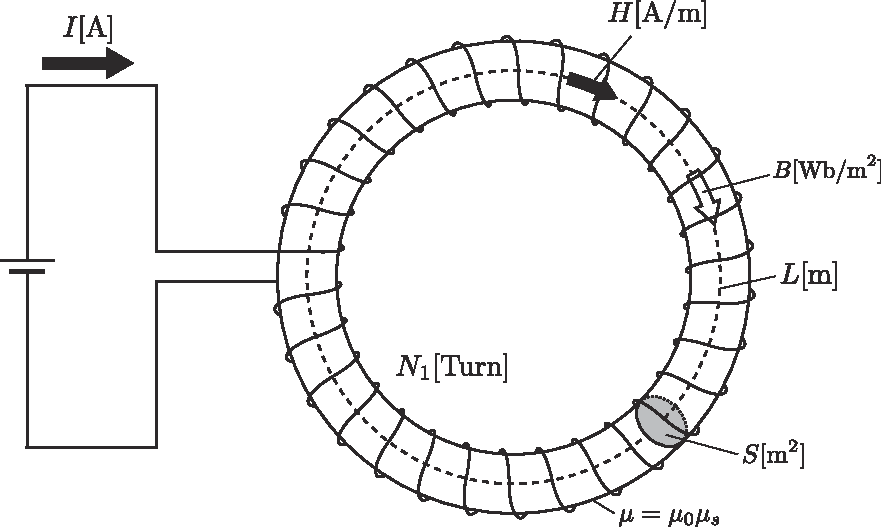
\includegraphics[width=70mm]{fig/magnetism_circuit.pdf}
	\caption{磁気回路}
	\label{fig:hys:jikikairo}
\end{figure}

鉄心の磁化力$H$と磁束密度$B$との関係を示す曲線をB-H曲線といい、一般に\wfig{hys:bhcurve}(a)のような飽和特性になる。
また磁化力$H$を正負の方向に増減すると、\wfig{hys:bhcurve}(b)の様なヒステリシス曲線になる。
\begin{figure}[htbp]
	\centering
	\begin{tabular}{cc}
		\includegraphics[width=70mm]{fig/bhcurve.pdf} &
		\includegraphics[width=70mm]{fig/hysteresis.pdf}             \\
		(a) B-H 曲線                                    & (b) ヒステリシス曲線
	\end{tabular}
	\caption{B-H曲線とヒステリシス曲線}
	\label{fig:hys:bhcurve}
\end{figure}

\subsection{交流磁化特性}
\wfig{hys:transformer}の変圧器のように、鉄心に巻かれた巻数$N_1$のコイルに交流電圧$V_1$を加えると、鉄心中に交番磁束$\phi$を作るための電流(励磁電流)$i_0$が流れる。このとき磁束密度$B$と磁化力$H$との間にはヒステリシス特性があるため、励磁電流は\wfig{hys:hizumi}のようにひずみを生ずる。この現象を逆に利用して、励磁電流$i_0$と交番磁束$\phi$の波形をなんらかの方法で取り出し、オシロスコープのX軸に励磁電流$i_0$の波形、Y軸に交番磁束$\phi$の波形を入力すれば、オシロスコープの画面に鉄心のヒステリシス特性(B-H曲線)が描かれる。
\begin{figure}[htbp]
	\centering
	\includegraphics[width=140mm]{fig/transformer.pdf}
	\caption{変圧器の交流磁化特性測定回路}
	\label{fig:hys:transformer}
\end{figure}

励磁電流$i_0$の波形を直接取り出すのは難しいので、\wfig{hys:transformer}において励磁電流$i_0$が抵抗$R_h$を流れるときの電圧変化、すなわち
\begin{equation}
	V_h = i_0R_h
\end{equation}
として取り出す。また、交番磁束$\phi$は次の様にして取り出す。

\wfig{hys:transformer}において二次巻線$N_2$と鎖交する磁束の時間に対する変化が二次誘起電圧$e_2$として現れるから
\begin{equation}
	e_2 = -N_2\frac{d \phi}{dt}
	\label{eq:hys:e2}
\end{equation}
となり、\weq{hys:e2}を変形すると
\begin{equation}
	d \phi = \frac{1}{N_2}\times e_2\times dt
	\label{eq:hys:dphi}
\end{equation}
となるから、交番磁束$\phi$は\weq{hys:dphi}を積分すれば求まることとなる。すなわち、二次巻線に発生する電圧$e_2$を時間で積分すればよい。そこで二次側にCR積分回路を接続しコンデンサCの両端から$e_2$を積分した、交番磁束に比例した電圧をとりだす。

\begin{figure}[htb]
	%\begin{center}
	\centering
	\subfloat[ヒステリシス現象のない場合]{
		\includegraphics[width=115mm]{fig/hizumi_a.pdf}
	}
	\vspace{5mm}
	\subfloat[ヒステリシス現象のある場合]{
		\includegraphics[width=115mm]{fig/hizumi_b.pdf}
	}
	\caption{ヒステリシス現象}
	\label{fig:hys:hizumi}
	%\end{center}    
\end{figure}

\section{方法}
\subsection{使用器具}
今回の実験で使用した器具を表\ref{tab:使用器具}に示す。
\begin{table}[htbp]
	\centering
	\caption{使用器具}
	\begin{tabular}{lll}
	使用器具            & 製造元      & 型番          \\ \hline \hline
	電圧計             & YEW      & TYPE2013    \\ \hline
	電流計             & YOKOGAWA & TYPE2013    \\ \hline
	低力率用力率計         & YOKOGAWA & MODEL 2041  \\ \hline
	スライダートランス       & 東京理工舎    & RSA-2       \\ \hline
	オシロスコープ         & KEYSIGHT & MSO-X 2004A \\ \hline
	ヒステリシス曲線直視回路セット & 不明       & 不明          \\ \hline
	\end{tabular}
	\label{tab:使用器具}
	\end{table}


\subsection{実験手順}


\section{結果}
\section{考察}
\section{結論}

\begin{thebibliography}{9}%参考文献数が10以上の場合は9を99に変更
	%\bibitem{xxx}の引用を本文中で行うには\cite{xxx}と記述。
	\bibitem{a} 著者名, 書名,出版社,発行年.
\end{thebibliography}


\end{document}

